% --------------------------------------------------------------------------
% Template for DMRN 2021 paper; to be used with:
%          dmrn2021.sty  - DMRN 2021 LaTeX style file
% Adapted from dcase2016.sty
% --------------------------------------------------------------------------

\documentclass{article}
\usepackage{caption}
\usepackage{times,amsmath,graphicx,url,dmrn2020}
\usepackage{indentfirst}
\setlength{\parskip}{0.5em}

% smaller font size for captions
\captionsetup[figure]{font=footnotesize,labelfont=footnotesize}
\captionsetup[table]{font=footnotesize,labelfont=footnotesize}

% reduce blank space after figures
\setlength{\belowcaptionskip}{-10pt}

% Example definitions.
% --------------------
\def\defeqn{\stackrel{\triangle}{=}}
\newcommand{\symmat}[1]{{\mbox{\boldmath $#1$}}}

% roman numbering of sections
\renewcommand{\thesection}{\Roman{section}} 

% Title.
% --------------------
\title{Building style-aware neural MIDI synthesizers using simplified differential DSP approach}

% Single addresses (uncomment and modify for single-address case).
% --------------------
% \oneauthor
% {Given-name Family-name(Surname)\sthanks{Research supported by ABC Foundation.}}
% {Department/Research Institute, University, Country}
% {john@fictional.edu}

% Two addresses
% --------------------
\twoauthors
 {Sergey Grechin}
    {Infinite Album}
    {grechin.sergey@gmail.com}
 {Given-name Family-name (Surname)}
    {Department/Research Institute, University, Country}
    
\begin{document}
%\ninept
\tenpt
\maketitle

\begin{sloppy}
\begin{abstract}
We explore how simplified differential DSP approach can be used to build realistically sounding virtual MIDI-controllable monophonic synthesizers. The simplification involves directly using  MIDI data as input to the DDSP decoder. On top of that, we show how  incorporating additional style-based and temporal channels can be used to imitate various aspects of performance and improve realism.  We further demonstrate the results of applying the approach to the task of modelling the sound of electric guitar. The presented results were obtained with a model trained on less than 12 minutes of manually MIDI-annotated audio. The source code is released along with the prepared dataset.
\end{abstract}

\begin{keywords}
Deep Learning, DDSP, virtual synthesizers, MIDI
\end{keywords}

\section{Model architecture and inputs}
\label{sec:architecture_and_inputs}

The model was built on top of \cite{ddsp_simplified_repo} which in turn is a simplified version of original DDSP design \cite{ddsp}. In contrast to the original implementation, in our model audio is not directly used to produce inputs to the decoder. 
Instead, we use MIDI annotations to heurustically generate fundamental frequency curve (F0), loudness, additional timing signals ("distance from onset" , "distance to offset"), proposed in \cite{control-synthesis}, and arbitrary CC (continuous controller) values. CC values are used to capture various performance characteristics such as "openness" - the degree of how muted the guitar string is when plucked.
Additional inputs are passed through dedicated stacks of dense layers before being concatenated with the traditional DDSP decoder inputs.

\section{Dataset and results}
\label{sec:dataset_and_results}

For training, 12 minutes of playing chromatic scales on an electric guitar  were recorded. MIDI annotations were made manually with CC55 used to represent open (127) and muted (1) sound. For training, velocity values were obtained using A-weighted loudness-based approach proposed in \cite{control-synthesis}. On inference stage velocity was taken from the source MIDI.

We encorage the reader to visit the online supplement page \cite{online_supplement} to listen to the generated examples and access additional resources such as the source code and the dataset.

\section{Future research}
\label{sec:future_research}


We plan to research if other aspects of playing style can be captured using this approach, such as playing with chords. For that, we plan to add additional harmonic synth stacks with independently learnable parameters.

\begin{figure}[t]
  \centering
  \centerline{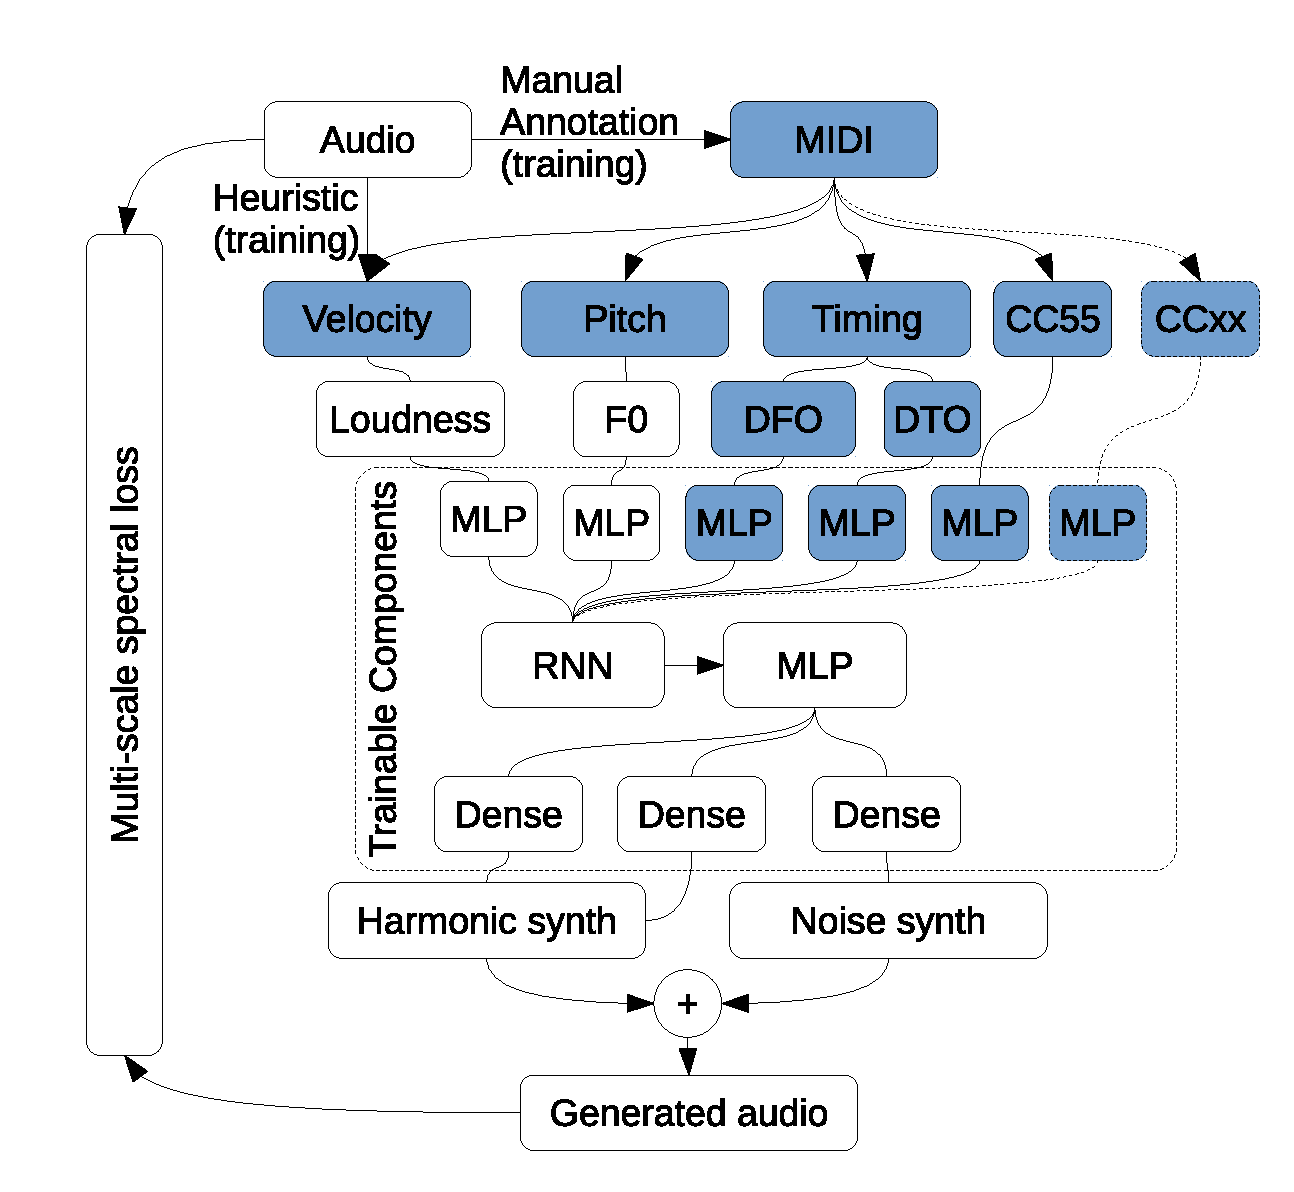
\includegraphics[scale=0.4]{components}}
  \caption{Componenets of the model. The white blocks represent the componements of original DDSP design \cite{ddsp}. 
MLP - Multilayer perceptron, 
DFO - distance from onset, 
DTO - distance to offset,
CC - continuous controller
}
  \label{fig:components}
\end{figure}

\begin{figure}[t]
  \centering
  \centerline{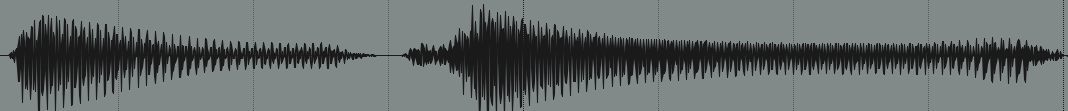
\includegraphics[scale=0.32]{generated_waveform}}
  \caption{Waveforms generated on C-5 for two MIDI notes with closed and open sound. This example demonstrates that the model has succeeded in learning temporal characteristics of the guitar sound, including the modelling of initial transient.}
  \label{fig:generated_waveform}
\end{figure}




% 
% ------------------------------------------------------------
% Either list references using the bibliography style file IEEEtran.bst

\bibliographystyle{IEEEtran}
{\footnotesize\bibliography{refs}}

% \bibliography{refs}
% how to deal with bibliography
% https://www.overleaf.com/learn/latex/Bibliography_management_with_bibtex

\end{sloppy}
\end{document}
